\documentclass[11pt]{article}
\usepackage[margin=0.9in]{geometry}
\usepackage[T1]{fontenc}
\usepackage{lmodern,microtype}
\usepackage{amsmath,amssymb,amsthm,mathtools}
\usepackage{booktabs,tabularx,array}
\usepackage{xcolor,graphicx,adjustbox,float}
\usepackage[numbers,sort&compress]{natbib}
\usepackage[colorlinks=true,linkcolor=blue!45!black,citecolor=blue!45!black,urlcolor=blue!45!black]{hyperref}
\usepackage{enumitem}
\setlist{nosep}
\newtheorem{proposition}{Proposition}
\newcommand{\R}{\mathbb R}
\newcommand{\sg}{\operatorname{sigmoid}}
\newcommand{\spplus}{\operatorname{softplus}}
% Generated by generate_results.py from the run records; do not edit.
\newcommand{\AlibiMqarDistSixtyFour}{0.0}
\newcommand{\AlibiMqarLoadEight}{38.0}
\newcommand{\AlibiPasskeyDistSixtyFour}{16.6}
\newcommand{\AlibiPasskeyLoadEight}{20.8}
\newcommand{\CtrlMqarDistSixtyFour}{47.8}
\newcommand{\CtrlMqarLoadEight}{9.3}
\newcommand{\CtrlPasskeyDistSixtyFour}{48.6}
\newcommand{\CtrlPasskeyLoadEight}{14.4}
\newcommand{\NopeMqarDistSixtyFour}{22.1}
\newcommand{\NopeMqarLoadEight}{7.6}
\newcommand{\NopePasskeyDistSixtyFour}{43.3}
\newcommand{\NopePasskeyLoadEight}{8.8}
\newcommand{\RopeMqarDistSixtyFour}{0.0}
\newcommand{\RopeMqarLoadEight}{0.4}
\newcommand{\RopePasskeyDistSixtyFour}{8.3}
\newcommand{\RopePasskeyLoadEight}{20.7}
\newcommand{\RopeYarnMqarDistSixtyFour}{74.3}
\newcommand{\RopeYarnMqarLoadEight}{83.6}
\newcommand{\RopeYarnPasskeyDistSixtyFour}{68.6}
\newcommand{\RopeYarnPasskeyLoadEight}{21.4}
\newcommand{\YarnFtMqarDistSixtyFour}{94.9}
\newcommand{\YarnFtMqarLoadEight}{37.9}
\newcommand{\YarnFtPasskeyDistSixtyFour}{96.0}
\newcommand{\YarnFtPasskeyLoadEight}{23.0}
\newcommand{\alibiCopyDistTwo}{76.4}
\newcommand{\alibiSelDistTwo}{37.5}
\newcommand{\bankPasskeyMem}{0.85}
\newcommand{\bankPasskeySwaMem}{0.74}
\newcommand{\bestBaseScaleDistSixtyFour}{38.5}
\newcommand{\bestBaseScaleLoadEight}{53.8}
\newcommand{\bestSelDistTwo}{37.5}
\newcommand{\ctrlParams}{82,881}
\newcommand{\extBaselineMax}{32}
\newcommand{\extMemOneMMax}{100}
\newcommand{\extMemOneMMin}{96}
\newcommand{\extMemOneMSec}{72}
\newcommand{\extMemOneMSeeds}{100, 96, 100}
\newcommand{\extNopeOneM}{10}
\newcommand{\extSwaMemHalfM}{74, 42, 50}
\newcommand{\frontSolveSteps}{2,000}
\newcommand{\infiniCopyDistTwo}{98.4}
\newcommand{\infiniSelDistTwo}{22.1}
\newcommand{\lmAlibiBpc}{1.426}
\newcommand{\lmAlibiFirst}{1.34}
\newcommand{\lmAlibiLast}{1.37}
\newcommand{\lmCtrlBpc}{2.01}
\newcommand{\lmCtrlFirst}{1.95}
\newcommand{\lmCtrlLast}{5.52}
\newcommand{\lmInfiniFirst}{1.48}
\newcommand{\lmInfiniLast}{1.62}
\newcommand{\lmMemBpc}{1.444}
\newcommand{\lmMemFirst}{1.35}
\newcommand{\lmMemLast}{3.26}
\newcommand{\lmMemPkOne}{68}
\newcommand{\lmNopeBpc}{3.12}
\newcommand{\lmRopeBpc}{1.450}
\newcommand{\lmRopeLast}{4.67}
\newcommand{\lmRopeYarnLast}{2.55}
\newcommand{\lmSwaFirst}{1.57}
\newcommand{\lmSwaLast}{1.83}
\newcommand{\lmSwaMemBpc}{1.472}
\newcommand{\lmSwaMemFirst}{1.39}
\newcommand{\lmSwaMemLast}{1.94}
\newcommand{\memCopyDistTwo}{61.0}
\newcommand{\memCopyVal}{99.7}
\newcommand{\memMqarDistSixtyFour}{96.9}
\newcommand{\memMqarLoadEight}{100.0}
\newcommand{\memParamFrac}{2.9}
\newcommand{\memParams}{82,839}
\newcommand{\memPasskeyDistSixtyFour}{100.0}
\newcommand{\memPasskeyLoadEight}{26.0}
\newcommand{\memScaleDistSixtyFour}{95.6}
\newcommand{\memScaleLoadEight}{99.9}
\newcommand{\memSelDistTwo}{31.6}
\newcommand{\memSelVal}{99.6}
\newcommand{\middleSolveSteps}{13,000--29,000}
\newcommand{\nopeScaleDistSixtyFour}{15.7}
\newcommand{\nopeScaleVal}{99.7}
\newcommand{\placeBackDistSixtyFour}{2.2}
\newcommand{\placeBackLoadEight}{6.6}
\newcommand{\placeCtrlMiddleDistSixtyFour}{22.1}
\newcommand{\placeCtrlMiddleLoadEight}{12.7}
\newcommand{\placeMiddleDistSixtyFour}{75.0}
\newcommand{\placeMiddleLoadEight}{23.2}
\newcommand{\placeSwaMiddleDistSixtyFour}{71.7}
\newcommand{\placeSwaMiddleLoadEight}{99.8}
\newcommand{\runsTotal}{459}
\newcommand{\swaMemCopyVal}{48.6}
\newcommand{\swaMemMqarDistSixtyFour}{96.9}
\newcommand{\swaMemPasskeyDistSixtyFour}{73.9}
\newcommand{\swaMemScaleDistSixtyFour}{96.8}
\newcommand{\swaMemSelVal}{93.9}
\newcommand{\xTwoDistSixtyFour}{100.0}


\title{Attention is My Memory:\\Positional Encoding-free Length Invariance in Transformers}
\author{Nicholas Rosdahl\\Independent Researcher}
\date{2026\\[0.5em]\small\href{https://doi.org/10.5281/zenodo.24268811}{doi:10.5281/zenodo.24268811}}

\begin{document}
\maketitle

\begin{abstract}
Every transformer inherits two limits from the way it represents order: a
\emph{context cap}, a maximum length fixed by its positional scheme and training
length, and a failure of \emph{length generalization}, the collapse of learned
behaviour on sequences longer than those seen in training. We remove positional
encoding entirely and insert a single memory, the admitted read of
DABSN~\citep{rosdahl2026dabsn}, once into the transformer. The memory is a thin
interface of four scalar tags and two projections feeding the original read
unchanged. Nothing in the resulting model is indexed by position, so it has no
architectural limit on sequence length. Trained on 256-token sequences, it keeps
\memMqarDistSixtyFour\% accuracy on multi-query associative recall at $64\times$
the training length and \memMqarLoadEight\% at $8\times$ the number of stored pairs,
where the strongest positional baseline, rotary embeddings fine-tuned with YaRN,
reaches \YarnFtMqarDistSixtyFour\% and \YarnFtMqarLoadEight\%. It retrieves a passkey
at $2^{20}$ tokens, $4096\times$ its training length, with
\extMemOneMMin--\extMemOneMMax\% digit accuracy across seeds, where the same
transformer without the memory scores \extNopeOneM\%. The result holds at a larger
width and depth. On character-level language modelling, the memory model without
any positional encoding matches positional transformers at the training length
(\lmMemBpc{} bits per character against \lmRopeBpc{} for rotary and \lmAlibiBpc{} for
ALiBi). All results come from one declared protocol of \runsTotal{} runs with
per-model learning-rate sweeps, three seeds, and the published task generators.
\end{abstract}

\section{Introduction}
\label{sec:intro}

Self-attention is permutation-equivariant: without additional machinery, it cannot
tell one ordering of its inputs from another~\citep{vaswani2017attention}. The
standard remedy is to inject position. Absolute embeddings attach a learned or
fixed vector to each index, rotary embeddings rotate queries and keys by an angle
proportional to position~\citep{su2021roformer}, and linear biases penalize
attention by distance~\citep{press2022train}. Each choice works within the lengths
it was trained on. Each also ties the model to those lengths.

The tie produces two distinct limits. The first is a \emph{context cap}: a learned
absolute table has no entry beyond its last index, and a rotary model meets
rotation angles it has never seen. The second is a failure of \emph{length
generalization}: even where a longer input is admissible, behaviour learned on
short sequences degrades on long ones~\citep{press2022train,kazemnejad2023impact}.
A large body of work extends context windows after training by interpolating or
rescaling positions~\citep{chen2023extending,peng2024yarn}. These methods move the
cap; they do not remove it, and the strongest of them require further training at
the new length.

Removing position altogether is not by itself a solution. Causal transformers with
no positional encoding (NoPE) still learn positional information
implicitly~\citep{haviv2022transformer} and can generalize better than positional
schemes on some tasks~\citep{kazemnejad2023impact}. But softmax attention over an
ever-growing sequence spreads its mass across more and more tokens, and retrieval
that was sharp at the training length is diluted beyond it. In our experiments a
NoPE transformer that learns associative recall at 256 tokens (\nopeScaleVal\%)
keeps \nopeScaleDistSixtyFour\% of it at $64\times$ that length.

We take a different route. DABSN~\citep{rosdahl2026dabsn} introduced an
\emph{admitted read}: a memory whose writes are admitted by content, addressed by
content, and retrieved by three primitives (content, permanent, and induction),
with no positional table of any kind. In a recurrent block, this read generalized
copying to $50\times$ the training length, a flatness that work attributes to
addressing that depends on no position~\citep{rosdahl2026dabsn}. This
paper asks whether the same read, used as the memory of a transformer that has no
positional encoding, removes the transformer's limits.

It removes the cap, and on retrieval it removes the length cliff. Our contributions are:
\begin{itemize}
\item \textbf{One memory, one interface.} We expose the admitted read through a
thin host interface: four scalar tags and two projections computed from the
transformer's hidden state (Section~\ref{sec:method}). The read itself is used
unchanged. It adds \memParams{} parameters (\memParamFrac\% of the base model), and a
single instance suffices.
\item \textbf{No context cap.} The model contains no position index, so no input
length is out of range (Proposition~\ref{prop:free}). Trained on 256 tokens, it
retrieves a passkey at $2^{20}$ tokens with \extMemOneMSeeds\% digit accuracy across
three seeds (Section~\ref{sec:extreme}).
\item \textbf{Length generalization of recall.} On multi-query associative recall and
passkey retrieval, accuracy holds as both the distance to the stored facts and the
number of facts grow. The strongest positional scheme, YaRN with fine-tuning at
$4\times$ the length, comes close on distance (\YarnFtMqarDistSixtyFour\% against
\memMqarDistSixtyFour\% at $64\times$) but holds \YarnFtMqarLoadEight\% of the facts at
$8\times$ the load, against \memMqarLoadEight\% (Section~\ref{sec:distance}). The result
holds at a larger width and depth (Section~\ref{sec:scale}).
\item \textbf{Placement.} With the memory at the front of the stack, the model solves
associative recall in \frontSolveSteps{} steps on every seed, against
\middleSolveSteps{} with the memory in the middle, and extrapolates further
(Section~\ref{sec:placement}).
\item \textbf{A complete protocol.} \runsTotal{} runs: every model is tuned on every
task, compared only where it learns the task, trained with three seeds, and
evaluated on byte-identical sequences generated by the published task code
(Section~\ref{sec:setup}).
\end{itemize}

\section{Background}
\label{sec:background}

\paragraph{Positional schemes and extrapolation.}
Rotary embeddings~\citep{su2021roformer} encode relative position through
rotations of query and key pairs. Beyond the training length, the model meets
rotation angles outside its training distribution. Attention with linear biases
(ALiBi)~\citep{press2022train} subtracts a head-specific penalty proportional to
distance, which keeps perplexity stable at longer lengths but suppresses access to
distant tokens by construction. Position interpolation~\citep{chen2023extending}
and YaRN~\citep{peng2024yarn} rescale rotary frequencies so that longer contexts
map into the trained range, usually followed by fine-tuning at the target length.
All of these keep position as the basis of addressing.

\paragraph{Transformers without positional encoding.}
A causal mask alone breaks permutation symmetry, and NoPE transformers recover
positional information from it~\citep{haviv2022transformer}. NoPE can
length-generalize better than explicit schemes on algorithmic
tasks~\citep{kazemnejad2023impact}, but its attention still spreads across all
preceding tokens. Sliding-window attention~\citep{beltagy2020longformer} bounds
each token's attention span and removes any limit on sequence length, at the price
of losing all access beyond the window.

\paragraph{Memory-augmented transformers.}
Memorizing Transformers~\citep{wu2022memorizing} retrieve past keys and values
with $k$-nearest-neighbour search. The Recurrent Memory
Transformer~\citep{bulatov2022recurrent} passes memory tokens between segments.
Landmark attention~\citep{mohtashami2023landmark} inserts block-summary tokens
that gate retrieval of whole blocks. Infini-attention~\citep{munkhdalai2024leave}
adds a compressive linear-attention memory to each attention layer. Each of these
retains positional machinery in the host, and each stores history by
\emph{arrival}: whatever passes through is kept, compressed, or summarized. The
memory studied here differs on both counts. The host carries no positional
encoding at all, and writes enter memory only if they are \emph{admitted by
content}.

\paragraph{Recall and induction.}
Multi-query associative recall (MQAR) measures a model's ability to retrieve the
value bound to a key presented earlier, and separates architectures that store
history exactly from those that compress it~\citep{arora2024zoology}. Induction
heads, the attention circuit that finds a previous occurrence of the current token
and copies its successor~\citep{olsson2022context}, are a central mechanism of
in-context learning. The admitted read implements induction directly as one of its
three primitives~\citep{rosdahl2026dabsn}.

\section{Method}
\label{sec:method}

\subsection{The admitted read}

We use the admitted read of DABSN exactly as defined in~\citep{rosdahl2026dabsn}
and summarize it here. The read consumes, at each position $t$, a query expression
$q_t\in\R^H$, a write $m_t\in\R^H$, and four scalar tags: novelty $\bar n_t$,
plasticity $\bar p_t$, energy $\bar e_t$, and saturation $\bar c_t$. Each write
receives an admission score
\begin{equation}
\mathrm{adm}_t = \gamma_p\log(1+H\bar p_t) + \gamma_n\bar n_t + \gamma_c\bar c_t
 + \gamma_e\bar e_t + \gamma_0,
\end{equation}
and is admitted when it lies within a learned window of the best score seen so far:
\begin{equation}
\mathrm{member}_t = \Big[\,\mathrm{adm}_t \ge \max_{k\le t}\mathrm{adm}_k
 - \spplus(w)\,\Big].
\label{eq:admission}
\end{equation}
The window is relative, so the admitted set adapts to the task and never collapses
to a single write. Over the admitted set, one score between the normalized query
and write,
$\mathrm{scale}\cdot(\hat q_i\cdot\hat m_j)+\mathrm{keybias}_j+\mathrm{adm}_j$,
is shared by three causal softmax reads: the \emph{content} and \emph{permanent}
reads gather the matched write itself, the latter adding a similarity between tag
signatures; the \emph{induction} read, over strictly earlier entries, gathers the
matched write's successor $m_{j+1}$, which is the copy primitive. The three are
combined with learned gains. A slow prediction-error trace accumulates writes whose
content departs from their recent expectation and is added to the read output with
a learned gain. None of these quantities contains a position index. Order enters
only through causality: the causal masks and the left-to-right trace.

\subsection{A host interface}

A transformer supplies none of these quantities natively. We derive them from the
host's hidden state $h_t\in\R^H$ at the insertion point with three feed-forward
maps:
\begin{align}
(\bar n_t,\bar p_t,\bar e_t,\bar c_t) &= \sg(W_\tau h_t+b_\tau),\\
q_t &= W_q h_t, \qquad m_t = \bar p_t\, W_m h_t.
\end{align}
The write follows DABSN's own contract, in which plasticity scales what is
written. $W_q$ and $W_m$ are initialized to the identity, so at initialization
the memory reads and writes the host's own representation. The tags are scalars:
the read consumes them only through their mean over hidden units, so no
$H$-wide tag vectors are stored. The read's recurrent-state inputs are set to zero,
so the memory branch carries retrieved content only and never re-emits the host
state. The only change to the read is the initial value of its admission window
(Eq.~\ref{eq:admission}), $\spplus(w)=1.5$, calibrated to the score scale of
host-derived tags. The window remains a learned parameter.

\subsection{Placement}

The memory enters the host as a single residual branch,
$h \leftarrow h + \mathrm{Mem}(\mathrm{LN}(h))$. We place exactly one memory per model
(two only in one ablation) and study three positions: at the \emph{front}, before the first block, where the
memory reads the token embeddings; in the \emph{middle}, before block $L/2$; and at
the \emph{back}, after the last block. The attention layers carry no positional
encoding. They are either full causal attention (NoPE + memory) or causal
sliding-window attention (sliding window + memory).

\subsection{Why there is no context cap}

\begin{proposition}[Position-free computation]
\label{prop:free}
Let the host transformer use no positional encoding. Then every quantity the
model computes at position $t$ is a function of the token contents at positions
$\le t$ and of the attention mask (causal, or causal and windowed), and of no
position index.
\end{proposition}

It follows that no parameter of the model is indexed by, or calibrated to, a
sequence length, and no input length is out of range. What can still change with
length is the \emph{distribution} of the quantities the model computes. That is an
empirical question, and the rest of the paper answers it.

\section{Experimental setup}
\label{sec:setup}

\paragraph{Tasks.} Every task uses its published generator; only the sequence length
is set by our protocol, with training at 256 tokens. \emph{MQAR} follows \texttt{multiquery\_ar} of~\citet{arora2024zoology}:
vocabulary 8192, keys from the lower half and values from the upper half, the
key--value block first, then the keys queried at power-law gaps with uniform random
tokens elsewhere; training mixes Zoology's three 256-token configurations (16, 32
and 64 pairs). \emph{Copying}~\citep{arjovsky2016unitary} and \emph{selective
copying}~\citep{gu2023mamba} use \texttt{torch\_copying\_data} from the S4
repository~\citep{gu2022efficiently}: 10 tokens over 8 symbols for copying, and
for selective copying the setting of~\citet{gu2023mamba}, 16 tokens at random
positions in a 16-token vocabulary, at our training length of 256 rather than their
4096. \emph{Passkey retrieval} uses the prompt
of~\citet{mohtashami2023landmark}, tokenized by word, with a uniform key in
$[1,50000]$ at a uniform depth; its digits are predicted.

\paragraph{Test axes.} \emph{Distance} holds the content at the largest training load
and inserts each task's own filler between the facts and their use, at $1\times$ to
$64\times$ the training length: uniform random tokens for MQAR
(excluding the sequence's keys, so every query keeps one answer), the noise token for
copying, the garbage text for passkey. \emph{Load} raises the number of items with
the filler at its training size; for MQAR this reproduces Zoology's test
configurations (512 tokens with 128 pairs, 1024 with 256) and extends them to 2048
with 512. Every model sees byte-identical evaluation sequences, derived from a fixed
seed, the axis, its value and the sample index: 256 validation sequences drawn like
the training data, and 128 test sequences per point.

\paragraph{Models.} All synthetic models are pre-LayerNorm decoder-only transformers
with width 128, 4 layers, 4 heads and an MLP ratio of 4. Baselines: NoPE; RoPE,
evaluated as trained and with position interpolation and YaRN applied at test time;
RoPE fine-tuned with YaRN, the standard recipe of~\citet{peng2024yarn}, in which each
converged RoPE model is trained for 2000 further steps at $4\times$ the length with
YaRN scaling and its selected learning rate; ALiBi; sliding-window NoPE (window 64);
Infini-attention~\citep{munkhdalai2024leave} in every layer (segment 64, rotary positions
within each segment, delta-rule memory; our implementation, as no official code exists); and a parameter-matched
control, a two-layer MLP with the memory's parameter count (\ctrlParams{} against
\memParams) in the memory's place. The memory models are NoPE + memory and sliding
window + memory. A larger tier repeats MQAR at width 256 with 8 layers and 8 heads.

\paragraph{Training.} AdamW~\citep{loshchilov2019decoupled} with
$\beta=(0.9,0.95)$, weight decay 0.1 on attention, MLP and output matrices only (the
memory and the matched control alike are not decayed), gradient clipping at 1.0,
bf16 autocast, batch 64. The rate is constant after a 200-step warmup, and training
stops once held-out validation accuracy reaches 99\% at two consecutive checks (one
check every 1000 steps), or at 30{,}000 steps. Every check is logged.

\paragraph{Selection.} Every model is trained on every task at rates
$\{3\times10^{-4},10^{-3},3\times10^{-3}\}$ with seed 0. If the best rate lies at an
edge of the grid without solving the task, one further rate past that edge
($10^{-4}$ or $10^{-2}$, Zoology's sweep range) is trained and joins the selection.
The rate with the best in-distribution validation accuracy is used for seeds 1 and 2;
test axes are never used for selection. A model is compared beyond the training
length only if it learns the task, i.e.\ reaches 90\% validation accuracy.
Table~\ref{tab:lr} lists the selected rates.

\paragraph{Language model.} Character-level enwik8~\citep{mahoney2011large} with the
standard 90M/5M/5M split; width 256, 6 layers, 8 heads, window 128; trained at 512
characters, batch 32, 20{,}000 steps with a cosine schedule; rates swept over 4000
steps at $\{3\times10^{-4},10^{-3},2\times10^{-3}\}$ with the same edge rule
($10^{-4}$ or $4\times10^{-3}$) and selected by validation loss; three seeds.

\section{Results}
\label{sec:results}

\subsection{Distance and load}
\label{sec:distance}

\begin{figure}[t]
\centering
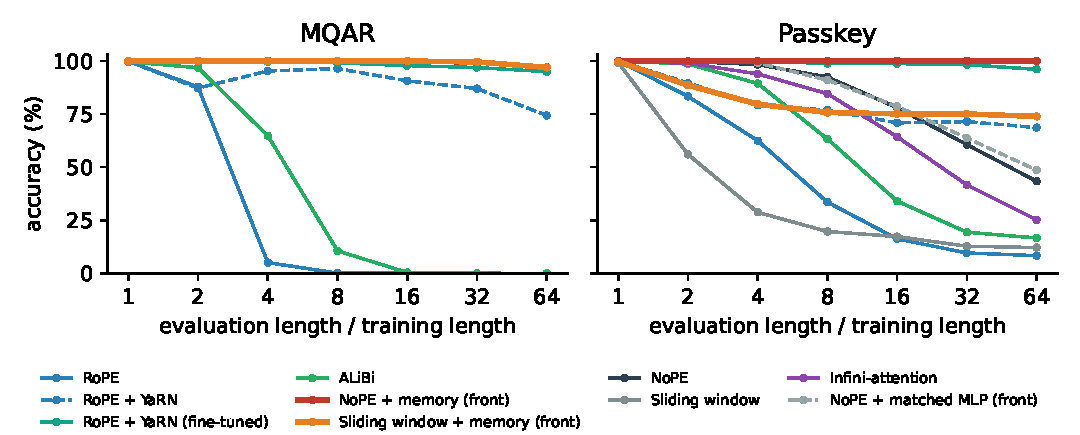
\includegraphics[width=\linewidth]{figs/distance.pdf}
\caption{Accuracy against evaluation length for the models that learn each task
(means over three seeds). RoPE + YaRN is applied at test time; the fine-tuned YaRN
model is trained at $4\times$ the length.}
\label{fig:distance}
\end{figure}

Tables~\ref{tab:mqar} and~\ref{tab:passkey} and Figure~\ref{fig:distance} show the
two retrieval tasks. On MQAR, both memory models hold \memMqarDistSixtyFour\% at
$64\times$ the training length and \memMqarLoadEight\% with $8\times$ the pairs. Every
positional scheme falls short along at least one axis. RoPE collapses beyond its training
length (\RopeMqarDistSixtyFour\% at $64\times$); YaRN at test time recovers part of
the distance axis (\RopeYarnMqarDistSixtyFour\%); ALiBi learns the task and then
suppresses distant facts by construction (\AlibiMqarDistSixtyFour\%). The strongest
baseline, RoPE fine-tuned with YaRN at $4\times$ the length, reaches
\YarnFtMqarDistSixtyFour\% on distance but \YarnFtMqarLoadEight\% on load: training at a
longer length extends the reach of its positions, not the number of facts it can
hold. The memory model, trained only at 256 tokens, does both. NoPE without the
memory does not reliably learn MQAR, and neither does the parameter-matched control
in the memory's place, so the memory's contribution is not one of parameter count.
Sliding-window attention and Infini-attention do not learn the task at all.

On passkey retrieval, NoPE + memory is at \memPasskeyDistSixtyFour\% at every
distance through $64\times$, where NoPE alone falls to \NopePasskeyDistSixtyFour\%, RoPE
with YaRN at test time to \RopeYarnPasskeyDistSixtyFour\%, ALiBi to
\AlibiPasskeyDistSixtyFour\%, and fine-tuned YaRN to \YarnFtPasskeyDistSixtyFour\%.

\begin{table}\centering\small
\setlength{\tabcolsep}{4pt}
\begin{adjustbox}{max width=\linewidth}
\begin{tabular}{lrrrrrrr}
\toprule
 & \multicolumn{1}{c}{train} & \multicolumn{4}{c}{distance} & \multicolumn{2}{c}{load} \\
Model & val & 1$\times$ & 4$\times$ & 16$\times$ & 64$\times$ & 2$\times$ & 8$\times$ \\
\midrule
NoPE$^\dagger$ & 67.9{\scriptsize$\pm$27.4} & 61.9{\scriptsize$\pm$32.6} & 45.9{\scriptsize$\pm$9.0} & 27.0{\scriptsize$\pm$18.7} & 22.1{\scriptsize$\pm$18.9} & 42.7{\scriptsize$\pm$28.0} & 7.6{\scriptsize$\pm$0.3} \\
RoPE & 99.8{\scriptsize$\pm$0.2} & 99.8{\scriptsize$\pm$0.3} & 5.0{\scriptsize$\pm$1.5} & 0.1{\scriptsize$\pm$0.1} & 0.0{\scriptsize$\pm$0.0} & 78.2{\scriptsize$\pm$16.4} & 0.4{\scriptsize$\pm$0.3} \\
RoPE + PI & 99.8{\scriptsize$\pm$0.2} & 99.8{\scriptsize$\pm$0.3} & 4.4{\scriptsize$\pm$5.3} & 1.4{\scriptsize$\pm$0.5} & 1.4{\scriptsize$\pm$0.6} & 37.2{\scriptsize$\pm$33.8} & 0.5{\scriptsize$\pm$0.4} \\
RoPE + YaRN & 99.8{\scriptsize$\pm$0.2} & 99.8{\scriptsize$\pm$0.3} & 95.2{\scriptsize$\pm$5.1} & 90.6{\scriptsize$\pm$1.9} & 74.3{\scriptsize$\pm$2.1} & 81.4{\scriptsize$\pm$29.8} & 83.6{\scriptsize$\pm$13.0} \\
RoPE + YaRN (fine-tuned) & 99.6{\scriptsize$\pm$0.5} & 99.5{\scriptsize$\pm$0.7} & 99.6{\scriptsize$\pm$0.5} & 97.8{\scriptsize$\pm$2.6} & 94.9{\scriptsize$\pm$5.7} & 73.0{\scriptsize$\pm$8.2} & 37.9{\scriptsize$\pm$10.9} \\
ALiBi & 99.6{\scriptsize$\pm$0.0} & 99.6{\scriptsize$\pm$0.2} & 64.8{\scriptsize$\pm$13.1} & 0.4{\scriptsize$\pm$0.2} & 0.0{\scriptsize$\pm$0.0} & 94.1{\scriptsize$\pm$8.4} & 38.0{\scriptsize$\pm$23.7} \\
Sliding window$^\dagger$ & 1.4{\scriptsize$\pm$0.1} & 1.0{\scriptsize$\pm$0.0} & 0.0{\scriptsize$\pm$0.0} & 0.0{\scriptsize$\pm$0.0} & 0.0{\scriptsize$\pm$0.0} & 0.2{\scriptsize$\pm$0.1} & 0.0{\scriptsize$\pm$0.0} \\
Infini-attention$^\dagger$ & 1.3{\scriptsize$\pm$0.4} & 0.8{\scriptsize$\pm$0.3} & 0.3{\scriptsize$\pm$0.1} & 0.1{\scriptsize$\pm$0.0} & 0.0{\scriptsize$\pm$0.0} & 0.3{\scriptsize$\pm$0.1} & 0.1{\scriptsize$\pm$0.0} \\
NoPE + matched MLP (front)$^\dagger$ & 60.7{\scriptsize$\pm$6.4} & 50.6{\scriptsize$\pm$8.7} & 48.6{\scriptsize$\pm$8.6} & 48.9{\scriptsize$\pm$8.3} & 47.8{\scriptsize$\pm$8.2} & 32.5{\scriptsize$\pm$8.5} & 9.3{\scriptsize$\pm$3.4} \\
\textbf{NoPE + memory (front)} & 100.0{\scriptsize$\pm$0.0} & \textbf{100.0}{\scriptsize$\pm$0.0} & \textbf{100.0}{\scriptsize$\pm$0.0} & \textbf{99.9}{\scriptsize$\pm$0.2} & \textbf{96.9}{\scriptsize$\pm$2.8} & \textbf{100.0}{\scriptsize$\pm$0.0} & \textbf{100.0}{\scriptsize$\pm$0.0} \\
\textbf{Sliding window + memory (front)} & 100.0{\scriptsize$\pm$0.0} & \textbf{100.0}{\scriptsize$\pm$0.0} & \textbf{100.0}{\scriptsize$\pm$0.0} & \textbf{99.9}{\scriptsize$\pm$0.1} & \textbf{96.9}{\scriptsize$\pm$2.4} & \textbf{100.0}{\scriptsize$\pm$0.0} & \textbf{100.0}{\scriptsize$\pm$0.0} \\
\bottomrule
\end{tabular}
\end{adjustbox}
\caption{MQAR~\citep{arora2024zoology}, trained at 256 tokens. Accuracy (\%), mean $\pm$ standard deviation over three seeds. Distance: filler between the facts and their use at $k\times$ the training length; load: $k\times$ the largest training load with the filler at its training size. The best model that learned the task is in bold; $^\dagger$ marks models below 90\% at the training length, which are not compared beyond it.}
\label{tab:mqar}
\end{table}

\begin{table}\centering\small
\setlength{\tabcolsep}{4pt}
\begin{adjustbox}{max width=\linewidth}
\begin{tabular}{lrrrrrrr}
\toprule
 & \multicolumn{1}{c}{train} & \multicolumn{4}{c}{distance} & \multicolumn{2}{c}{load} \\
Model & val & 1$\times$ & 4$\times$ & 16$\times$ & 64$\times$ & 2$\times$ & 8$\times$ \\
\midrule
NoPE & 99.8{\scriptsize$\pm$0.2} & 99.9{\scriptsize$\pm$0.1} & 98.3{\scriptsize$\pm$1.9} & 78.0{\scriptsize$\pm$13.3} & 43.3{\scriptsize$\pm$11.5} & 50.0{\scriptsize$\pm$13.0} & 8.8{\scriptsize$\pm$7.3} \\
RoPE & 100.0{\scriptsize$\pm$0.0} & \textbf{100.0}{\scriptsize$\pm$0.0} & 62.4{\scriptsize$\pm$21.7} & 16.2{\scriptsize$\pm$10.7} & 8.3{\scriptsize$\pm$0.6} & 54.1{\scriptsize$\pm$7.0} & 20.7{\scriptsize$\pm$3.3} \\
RoPE + PI & 100.0{\scriptsize$\pm$0.0} & \textbf{100.0}{\scriptsize$\pm$0.0} & 33.8{\scriptsize$\pm$2.8} & 21.1{\scriptsize$\pm$2.8} & 15.0{\scriptsize$\pm$3.2} & 53.5{\scriptsize$\pm$10.4} & 18.2{\scriptsize$\pm$3.0} \\
RoPE + YaRN & 100.0{\scriptsize$\pm$0.0} & \textbf{100.0}{\scriptsize$\pm$0.0} & 79.1{\scriptsize$\pm$17.9} & 70.8{\scriptsize$\pm$27.0} & 68.6{\scriptsize$\pm$35.6} & 53.3{\scriptsize$\pm$6.8} & 21.4{\scriptsize$\pm$2.3} \\
RoPE + YaRN (fine-tuned) & 99.3{\scriptsize$\pm$1.2} & 99.8{\scriptsize$\pm$0.3} & \textbf{99.9}{\scriptsize$\pm$0.1} & 98.7{\scriptsize$\pm$2.2} & 96.0{\scriptsize$\pm$5.3} & 58.3{\scriptsize$\pm$4.2} & 23.0{\scriptsize$\pm$2.7} \\
ALiBi & 100.0{\scriptsize$\pm$0.0} & 99.9{\scriptsize$\pm$0.1} & 89.3{\scriptsize$\pm$14.3} & 34.0{\scriptsize$\pm$5.8} & 16.6{\scriptsize$\pm$4.6} & 64.1{\scriptsize$\pm$8.3} & 20.8{\scriptsize$\pm$4.9} \\
Sliding window & 98.9{\scriptsize$\pm$0.1} & 99.2{\scriptsize$\pm$0.4} & 28.7{\scriptsize$\pm$2.3} & 17.3{\scriptsize$\pm$1.1} & 12.1{\scriptsize$\pm$2.6} & 29.1{\scriptsize$\pm$7.7} & 10.4{\scriptsize$\pm$0.4} \\
Infini-attention & 100.0{\scriptsize$\pm$0.0} & 99.7{\scriptsize$\pm$0.6} & 93.9{\scriptsize$\pm$7.1} & 64.2{\scriptsize$\pm$10.6} & 25.2{\scriptsize$\pm$7.8} & 20.0{\scriptsize$\pm$2.3} & 7.6{\scriptsize$\pm$2.9} \\
NoPE + matched MLP (front) & 99.7{\scriptsize$\pm$0.4} & 99.7{\scriptsize$\pm$0.5} & 99.1{\scriptsize$\pm$0.4} & 78.6{\scriptsize$\pm$6.5} & 48.6{\scriptsize$\pm$15.2} & 48.6{\scriptsize$\pm$27.7} & 14.4{\scriptsize$\pm$1.2} \\
\textbf{NoPE + memory (front)} & 100.0{\scriptsize$\pm$0.0} & \textbf{100.0}{\scriptsize$\pm$0.0} & \textbf{99.9}{\scriptsize$\pm$0.1} & \textbf{100.0}{\scriptsize$\pm$0.0} & \textbf{100.0}{\scriptsize$\pm$0.0} & 74.8{\scriptsize$\pm$10.4} & 26.0{\scriptsize$\pm$3.5} \\
\textbf{Sliding window + memory (front)} & 99.8{\scriptsize$\pm$0.0} & 99.6{\scriptsize$\pm$0.2} & 79.6{\scriptsize$\pm$4.0} & 75.1{\scriptsize$\pm$5.1} & 73.9{\scriptsize$\pm$6.7} & \textbf{84.4}{\scriptsize$\pm$2.3} & \textbf{32.1}{\scriptsize$\pm$1.1} \\
\bottomrule
\end{tabular}
\end{adjustbox}
\caption{Passkey retrieval~\citep{mohtashami2023landmark}, trained at 256 tokens. Accuracy (\%), mean $\pm$ standard deviation over three seeds. Distance: filler between the facts and their use at $k\times$ the training length; load: $k\times$ the largest training load with the filler at its training size. The best model that learned the task is in bold; $^\dagger$ marks models below 90\% at the training length, which are not compared beyond it.}
\label{tab:passkey}
\end{table}


\subsection{Extreme length}
\label{sec:extreme}

\begin{figure}[t]
\centering
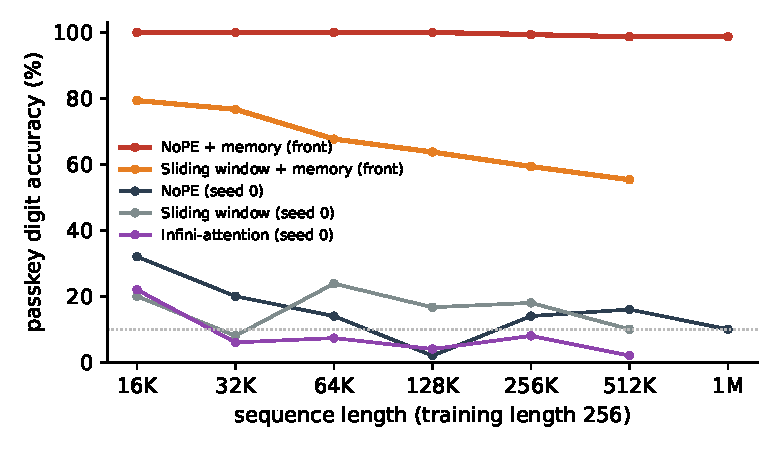
\includegraphics[width=0.72\linewidth]{figs/extreme.pdf}
\caption{Passkey retrieval from $16$K to $2^{20}$ tokens, trained at 256 (means over
the seeds in Table~\ref{tab:extreme}).}
\label{fig:extreme}
\end{figure}

The passkey checkpoints were evaluated at $2^{14}$ to $2^{20}$ tokens
(Table~\ref{tab:extreme}, Figure~\ref{fig:extreme}). NoPE + memory retrieves the
passkey at one million tokens with \extMemOneMSeeds\% digit accuracy on its three
seeds, $4096\times$ the length it was trained on. The same transformer without the
memory scores \extNopeOneM\% at that length, and no baseline exceeds
\extBaselineMax\% at any length from $16$K tokens on. Sliding window + memory, whose
attention sees only 64 tokens, still retrieves the key at $2^{19}$ tokens
(\extSwaMemHalfM\% on its three seeds). One forward pass of NoPE + memory over
$2^{20}$ tokens took about \extMemOneMSec~s on a single NVIDIA L4, with exact full
attention and an exact read.

\begin{table}\centering\small
\setlength{\tabcolsep}{4pt}
\begin{tabular}{llrrrrrrr}
\toprule
Model & Seed & 16K & 32K & 64K & 128K & 256K & 512K & 1M \\
\midrule
\textbf{NoPE + memory (front)} & 0 & 100 & 100 & 100 & 100 & 100 & 100 & 100 \\
\textbf{NoPE + memory (front)} & 1 & 100 & 100 & 100 & 100 & 98 & 98 & 96 \\
\textbf{NoPE + memory (front)} & 2 & 100 & 100 & 100 & 100 & 100 & 98 & 100 \\
\textbf{Sliding window + memory (front)} & 0 & 86 & 88 & 74 & 76 & 78 & 74 & --\rlap{$^\ast$} \\
\textbf{Sliding window + memory (front)} & 1 & 74 & 68 & 58 & 58 & 40 & 42 & --\rlap{$^\ast$} \\
\textbf{Sliding window + memory (front)} & 2 & 78 & 74 & 72 & 57 & 60 & 50 & --\rlap{$^\ast$} \\
NoPE & 0 & 32 & 20 & 14 & 2 & 14 & 16 & 10 \\
Sliding window & 0 & 20 & 8 & 24 & 17 & 18 & 10 & --\rlap{$^\ast$} \\
Infini-attention & 0 & 22 & 6 & 7 & 4 & 8 & 2 & --\rlap{$^\ast$} \\
\bottomrule
\end{tabular}
\caption{Passkey retrieval far beyond the 256-token training length: digit accuracy (\%) over 10 prompts per length (chance 10\%), on the passkey checkpoints of the main phase (every seed for the memory models, seed 0 for the baselines). $^\ast$The reference sliding-window and segment attention kernels used here exceed a CUDA launch limit at $2^{20}$ tokens (one call with $2^{16}$ attention blocks); no result exists for those models at that length.}
\label{tab:extreme}
\end{table}


\subsection{Scale}
\label{sec:scale}

At width 256 with 8 layers, with its own sweep and seeds (Table~\ref{tab:scale}), the
picture is unchanged: NoPE + memory holds \memScaleDistSixtyFour\% at $64\times$ and
\memScaleLoadEight\% at $8\times$ load (sliding window + memory
\swaMemScaleDistSixtyFour\% at $64\times$), against at most
\bestBaseScaleDistSixtyFour\% and \bestBaseScaleLoadEight\% for any positional
baseline. At this size NoPE learns the task in distribution, and its accuracy still
falls with distance and load; the memory is what holds it.

\begin{table}\centering\small
\setlength{\tabcolsep}{4pt}
\begin{adjustbox}{max width=\linewidth}
\begin{tabular}{lrrrrrrr}
\toprule
 & \multicolumn{1}{c}{train} & \multicolumn{4}{c}{distance} & \multicolumn{2}{c}{load} \\
Model & val & 1$\times$ & 4$\times$ & 16$\times$ & 64$\times$ & 2$\times$ & 8$\times$ \\
\midrule
NoPE & 99.7{\scriptsize$\pm$0.1} & 99.6{\scriptsize$\pm$0.0} & 91.5{\scriptsize$\pm$2.3} & 41.2{\scriptsize$\pm$9.5} & 15.7{\scriptsize$\pm$8.2} & 92.2{\scriptsize$\pm$3.5} & 23.5{\scriptsize$\pm$3.9} \\
RoPE & 99.7{\scriptsize$\pm$0.1} & 99.7{\scriptsize$\pm$0.1} & 0.5{\scriptsize$\pm$0.3} & 0.0{\scriptsize$\pm$0.0} & 0.0{\scriptsize$\pm$0.0} & 56.6{\scriptsize$\pm$8.7} & 0.1{\scriptsize$\pm$0.0} \\
RoPE + PI & 99.7{\scriptsize$\pm$0.1} & 99.7{\scriptsize$\pm$0.1} & 21.9{\scriptsize$\pm$10.6} & 2.8{\scriptsize$\pm$1.4} & 1.8{\scriptsize$\pm$1.1} & 79.2{\scriptsize$\pm$5.3} & 2.3{\scriptsize$\pm$1.5} \\
RoPE + YaRN & 99.7{\scriptsize$\pm$0.1} & 99.7{\scriptsize$\pm$0.1} & 89.6{\scriptsize$\pm$7.2} & 51.7{\scriptsize$\pm$9.3} & 38.5{\scriptsize$\pm$5.1} & 92.8{\scriptsize$\pm$2.1} & 47.2{\scriptsize$\pm$14.0} \\
ALiBi & 99.7{\scriptsize$\pm$0.1} & 99.6{\scriptsize$\pm$0.1} & 58.4{\scriptsize$\pm$4.8} & 0.0{\scriptsize$\pm$0.0} & 0.0{\scriptsize$\pm$0.0} & 98.8{\scriptsize$\pm$0.3} & 53.8{\scriptsize$\pm$3.5} \\
Sliding window$^\dagger$ & 2.1{\scriptsize$\pm$0.2} & 1.2{\scriptsize$\pm$0.0} & 0.0{\scriptsize$\pm$0.0} & 0.0{\scriptsize$\pm$0.0} & 0.0{\scriptsize$\pm$0.0} & 0.2{\scriptsize$\pm$0.0} & 0.0{\scriptsize$\pm$0.0} \\
Infini-attention$^\dagger$ & 2.1{\scriptsize$\pm$0.4} & 1.4{\scriptsize$\pm$0.4} & 0.3{\scriptsize$\pm$0.2} & 0.1{\scriptsize$\pm$0.0} & 0.0{\scriptsize$\pm$0.0} & 0.5{\scriptsize$\pm$0.2} & 0.1{\scriptsize$\pm$0.0} \\
\textbf{NoPE + memory (front)} & 99.9{\scriptsize$\pm$0.0} & \textbf{100.0}{\scriptsize$\pm$0.0} & \textbf{100.0}{\scriptsize$\pm$0.0} & \textbf{99.8}{\scriptsize$\pm$0.1} & 95.6{\scriptsize$\pm$2.6} & \textbf{100.0}{\scriptsize$\pm$0.0} & \textbf{99.9}{\scriptsize$\pm$0.0} \\
\textbf{Sliding window + memory (front)} & 100.0{\scriptsize$\pm$0.0} & \textbf{100.0}{\scriptsize$\pm$0.0} & \textbf{100.0}{\scriptsize$\pm$0.0} & \textbf{99.8}{\scriptsize$\pm$0.1} & \textbf{96.8}{\scriptsize$\pm$0.5} & \textbf{100.0}{\scriptsize$\pm$0.0} & \textbf{99.9}{\scriptsize$\pm$0.0} \\
\bottomrule
\end{tabular}
\end{adjustbox}
\caption{MQAR with width 256 and 8 layers, with its own learning-rate sweep and seeds. Accuracy (\%), mean $\pm$ standard deviation over three seeds. Distance: filler between the facts and their use at $k\times$ the training length; load: $k\times$ the largest training load with the filler at its training size. The best model that learned the task is in bold; $^\dagger$ marks models below 90\% at the training length, which are not compared beyond it.}
\label{tab:scale}
\end{table}


\subsection{Placement}
\label{sec:placement}

Table~\ref{tab:placement} places the single memory at the front, middle and back of
the stack on MQAR, with the matched control at the same place. The front is best on
every measure. It learns fastest, solving the task in \frontSolveSteps{} steps on
every seed against \middleSolveSteps{} in the middle, and it extrapolates furthest:
\memMqarDistSixtyFour\% at $64\times$ against \placeMiddleDistSixtyFour\% in the middle
and \placeBackDistSixtyFour\% at the back, and \memMqarLoadEight\% at $8\times$ load
against \placeMiddleLoadEight\% and \placeBackLoadEight\%. In the middle, the
sliding-window host still holds load (\placeSwaMiddleLoadEight\%). Every placement
learns the task at the training length; only the front and middle placements carry
it far beyond. A second memory at the back, added to the front one, reaches
\xTwoDistSixtyFour\% at $64\times$, against \memMqarDistSixtyFour\% for the front memory
alone: one memory suffices.

\begin{table}\centering\small
\setlength{\tabcolsep}{4pt}
\begin{adjustbox}{max width=\linewidth}
\begin{tabular}{lrrrrrrr}
\toprule
 & \multicolumn{1}{c}{train} & \multicolumn{4}{c}{distance} & \multicolumn{2}{c}{load} \\
Model & val & 1$\times$ & 4$\times$ & 16$\times$ & 64$\times$ & 2$\times$ & 8$\times$ \\
\midrule
NoPE + matched MLP (front)$^\dagger$ & 60.7{\scriptsize$\pm$6.4} & 50.6{\scriptsize$\pm$8.7} & 48.6{\scriptsize$\pm$8.6} & 48.9{\scriptsize$\pm$8.3} & 47.8{\scriptsize$\pm$8.2} & 32.5{\scriptsize$\pm$8.5} & 9.3{\scriptsize$\pm$3.4} \\
\textbf{NoPE + memory (front)} & 100.0{\scriptsize$\pm$0.0} & \textbf{100.0}{\scriptsize$\pm$0.0} & \textbf{100.0}{\scriptsize$\pm$0.0} & \textbf{99.9}{\scriptsize$\pm$0.2} & \textbf{96.9}{\scriptsize$\pm$2.8} & \textbf{100.0}{\scriptsize$\pm$0.0} & \textbf{100.0}{\scriptsize$\pm$0.0} \\
\textbf{Sliding window + memory (front)} & 100.0{\scriptsize$\pm$0.0} & \textbf{100.0}{\scriptsize$\pm$0.0} & \textbf{100.0}{\scriptsize$\pm$0.0} & \textbf{99.9}{\scriptsize$\pm$0.1} & \textbf{96.9}{\scriptsize$\pm$2.4} & \textbf{100.0}{\scriptsize$\pm$0.0} & \textbf{100.0}{\scriptsize$\pm$0.0} \\
NoPE + matched MLP (middle) & 92.0{\scriptsize$\pm$13.3} & 89.5{\scriptsize$\pm$17.8} & 65.0{\scriptsize$\pm$12.8} & 31.6{\scriptsize$\pm$28.1} & 22.1{\scriptsize$\pm$23.8} & 73.5{\scriptsize$\pm$22.1} & 12.7{\scriptsize$\pm$4.6} \\
\textbf{NoPE + memory (middle)} & 99.6{\scriptsize$\pm$0.2} & 99.5{\scriptsize$\pm$0.2} & 96.5{\scriptsize$\pm$0.9} & 90.7{\scriptsize$\pm$5.7} & 75.0{\scriptsize$\pm$18.8} & 88.6{\scriptsize$\pm$2.8} & 23.2{\scriptsize$\pm$2.8} \\
\textbf{Sliding window + memory (middle)} & 99.9{\scriptsize$\pm$0.1} & \textbf{100.0}{\scriptsize$\pm$0.0} & 99.9{\scriptsize$\pm$0.1} & 95.6{\scriptsize$\pm$4.8} & 71.7{\scriptsize$\pm$26.6} & \textbf{100.0}{\scriptsize$\pm$0.0} & 99.8{\scriptsize$\pm$0.3} \\
\textbf{NoPE + memory (back)} & 99.8{\scriptsize$\pm$0.2} & 99.8{\scriptsize$\pm$0.2} & 52.9{\scriptsize$\pm$30.4} & 8.1{\scriptsize$\pm$8.2} & 2.2{\scriptsize$\pm$3.1} & 76.5{\scriptsize$\pm$2.0} & 6.6{\scriptsize$\pm$4.8} \\
\bottomrule
\end{tabular}
\end{adjustbox}
\caption{Placement of the single memory on MQAR, with the parameter-matched control at the same place. Accuracy (\%), mean $\pm$ standard deviation over three seeds. Distance: filler between the facts and their use at $k\times$ the training length; load: $k\times$ the largest training load with the filler at its training size. The best model that learned the task is in bold; $^\dagger$ marks models below 90\% at the training length, which are not compared beyond it.}
\label{tab:placement}
\end{table}


\subsection{Copying and selective copying}
\label{sec:copy}

Except for the two sliding-window models, every model trained at 256 tokens learns
copying there (Table~\ref{tab:copy}). Beyond it, NoPE + memory keeps \memCopyDistTwo\%
at $2\times$, above NoPE, every RoPE variant and the matched control, while
Infini-attention (\infiniCopyDistTwo\%) and ALiBi (\alibiCopyDistTwo\%) extrapolate
further. Sliding window + memory does not learn copying at the training length
(\swaMemCopyVal\%). Selective copying is learned at 256 tokens by every model trained there
except plain sliding-window attention, and extrapolated by none: the best model at
$2\times$ reaches \bestSelDistTwo\% (Table~\ref{tab:selcopy}).
Section~\ref{sec:discussion} returns to these two tasks.

\subsection{Language modelling}
\label{sec:lm}

\begin{figure}[t]
\centering
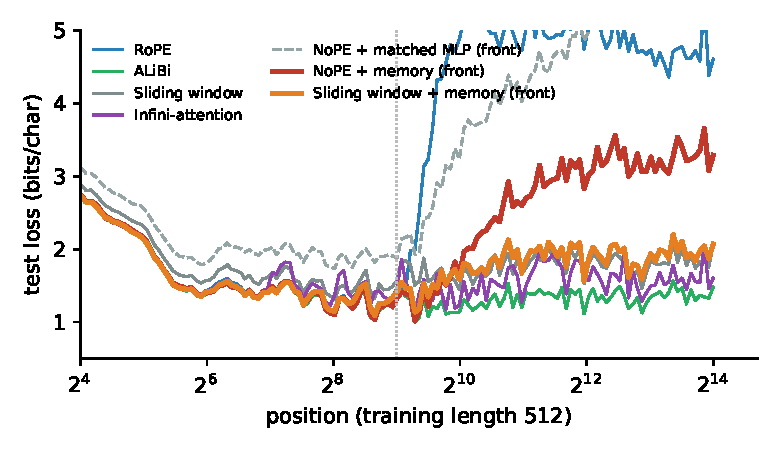
\includegraphics[width=0.72\linewidth]{figs/lm_position.pdf}
\caption{enwik8 test loss by position over sequences of $32\times$ the training length
(means over three seeds; running mean over 32 positions). The dotted line marks the
training length.}
\label{fig:lm}
\end{figure}

On enwik8 (Table~\ref{tab:lm}, Figure~\ref{fig:lm}), NoPE + memory reaches
\lmMemBpc{} bits per character at the training length, level with the positional
models (RoPE \lmRopeBpc, ALiBi \lmAlibiBpc) and with sliding window + memory
(\lmSwaMemBpc), without any positional encoding. NoPE alone (\lmNopeBpc) and NoPE with
the matched MLP in the memory's place (\lmCtrlBpc) are far behind, so the memory is
what makes a position-free language model competitive. On the exact passkey prompt
of~\citet{mohtashami2023landmark} at the training length, NoPE + memory and ALiBi
lead at \lmMemPkOne\%.

Beyond the training length, the test loss of NoPE + memory rises from \lmMemFirst{} to
\lmMemLast{} bits per character at $16$--$32\times$. That is well below its matched
control (\lmCtrlFirst{} to \lmCtrlLast) and RoPE as trained (\lmRopeLast), but above
RoPE with YaRN at test time (\lmRopeYarnLast) and the models whose attention is
restricted to recent context: ALiBi stays flat (\lmAlibiFirst{} to \lmAlibiLast), and
sliding window + memory rises only to \lmSwaMemLast. On natural text at this
scale, the memory gives a position-free model language-modelling quality equal to
positional ones within the training length; holding that quality at many times the
training length is the open part of the language-modelling result.

\begin{table}\centering\small
\setlength{\tabcolsep}{3.5pt}
\begin{adjustbox}{max width=\linewidth}
\begin{tabular}{l r rrrrrr rrr}
\toprule
 & val & \multicolumn{6}{c}{test loss by position (bits/char)} & \multicolumn{3}{c}{passkey (\%)} \\
Model & bpc & 0--512 & 512--1K & 1K--2K & 2K--4K & 4K--8K & 8K--16K & $1\times$ & $4\times$ & $32\times$ \\
\midrule
NoPE & 3.117 & 3.17 & 3.38 & 3.61 & 3.74 & 3.97 & 3.94 & 4 & 6 & 3 \\
RoPE & 1.450 & 1.36 & 3.58 & 5.04 & 5.02 & 4.89 & 4.67 & 58 & 1 & 0 \\
RoPE + PI &  & 4.62 & 4.86 & 4.80 & 4.90 & 4.92 & 4.69 & 58 & 0 & 0 \\
RoPE + YaRN &  & 2.02 & 2.30 & 2.35 & 2.48 & 2.51 & 2.55 & 58 & 48 & 35 \\
ALiBi & 1.426 & 1.34 & 1.20 & 1.30 & 1.36 & 1.30 & 1.37 & 68 & 9 & 4 \\
Sliding window & 1.658 & 1.57 & 1.65 & 1.75 & 1.84 & 1.73 & 1.83 & 7 & 0 & 0 \\
Infini-attention & 1.563 & 1.48 & 1.39 & 1.54 & 1.65 & 1.57 & 1.62 & 6 & 1 & 1 \\
NoPE + matched MLP (front) & 2.012 & 1.95 & 2.69 & 4.04 & 4.69 & 5.34 & 5.52 & 22 & 4 & 1 \\
\textbf{NoPE + memory (front)} & 1.444 & 1.35 & 1.47 & 2.42 & 2.94 & 3.21 & 3.26 & 68 & 13 & 8 \\
\textbf{Sliding window + memory (front)} & 1.472 & 1.39 & 1.51 & 1.85 & 1.93 & 1.84 & 1.94 & 15 & 1 & 1 \\
\bottomrule
\end{tabular}
\end{adjustbox}
\caption{Character-level enwik8, trained at 512 characters; means over three seeds. Validation bits per character at the training length; test loss averaged over position ranges of 16 sequences of $32\times$ the training length; passkey digit accuracy on the exact prompt of~\citet{mohtashami2023landmark} at $k\times$ the training length (32 prompts each, chance 10\%).}
\label{tab:lm}
\end{table}


\section{Admission and cost}
\label{sec:cost}

The read's work is proportional to the sequence length times the size of the
admitted bank. Table~\ref{tab:bank} reports the bank as a fraction of the length,
measured one sequence at a time. With full attention in the host, the memory admits
almost every write on MQAR and copying, so its cost grows with the square of the
length, as attention's does; on passkey it admits \bankPasskeyMem{} of the length.
With a sliding-window host, admission is selective on passkey (\bankPasskeySwaMem{} at
$64\times$), copying and selective copying, and the fraction is set by the task, not
by the length: it is nearly the same at $1\times$ and $64\times$.

In memory, a sliding window + memory model holds the attention keys and values of
its last 64 tokens per layer plus the admitted writes, at most two $H$-wide vectors
per admitted entry (the write and its successor, for the induction read). A
full-attention transformer holds $2LH$ values per token across $L$ layers. At long
lengths the sliding window + memory model therefore needs at most $1/L$ of the state
of a full key--value cache, a quarter with $L=4$, and less where admission is
selective; its per-token state does not depend on the number of layers. NoPE +
memory keeps a full cache in addition to its bank. We report costs in these hardware-independent units; the reference implementation used
here processes $2^{20}$ tokens in about \extMemOneMSec~s on one L4
(Section~\ref{sec:extreme}).

\begin{table}\centering\small
\begin{tabular}{llrrrr}
\toprule
Task & Model & $1\times$ & $4\times$ & $16\times$ & $64\times$ \\
\midrule
MQAR & NoPE + memory (front) & 1.00 & 1.00 & 1.00 & 1.00 \\
MQAR & Sliding window + memory (front) & 1.00 & 1.00 & 1.00 & 1.00 \\
Passkey & NoPE + memory (front) & 0.85 & 0.85 & 0.85 & 0.85 \\
Passkey & Sliding window + memory (front) & 0.77 & 0.77 & 0.75 & 0.74 \\
Copying & NoPE + memory (front) & 1.00 & 1.00 & 1.00 & 1.00 \\
Copying & Sliding window + memory (front) & 0.68 & 0.67 & 0.67 & 0.67 \\
Selective copying & NoPE + memory (front) & 1.00 & 1.00 & 1.00 & 1.00 \\
Selective copying & Sliding window + memory (front) & 0.72 & 0.69 & 0.69 & 0.68 \\
\bottomrule
\end{tabular}
\caption{Admitted bank as a fraction of the sequence length, at $k\times$ the training length (8 sequences per point, read one at a time; mean over seeds).}
\label{tab:bank}
\end{table}


\section{Discussion}
\label{sec:discussion}

Positional encodings were introduced to give attention a sense of order. They also
gave it a ruler, and every ruler has an end. The memory studied here supplies order
differently. Within a context, causal attention and the causal mask provide local
structure. Across a context of any length, retrieval is by content. The resulting
model has no index to run out of, and on the retrieval tasks it does not need one:
it holds what it learned at 256 tokens at a million.

\paragraph{Placement is a choice of address.} At the front, the memory reads token
embeddings, so each write is addressed by the identity of a single token. That is
exactly the address MQAR and passkey need, and it is where the memory learned
fastest and generalized furthest. Copying and language modelling ask for a different
address. In copying, every marker token is identical, so at the front each marker
presents the same query to the memory, and order must come from the attention above
it. In character-level text, a single character is a weak address. In the middle of
the stack, attention has already placed each token in its context, so the write and
the query carry that context. The language model and the copying tasks were run with
the memory at the front only; whether a middle placement extends the
language-modelling and copying results the way the front placement extends recall is
the direct next experiment, and nothing in the interface prevents it.

\paragraph{Limitations.} The models are small: width 128 with 4 layers, a tier at
width 256 with 8 layers, and a 6-layer character-level language model. The language
model matches positional models within its training length but its loss rises beyond
it, unlike models with a recency bias. On copying, two baselines extrapolate further,
and no model extrapolates selective copying. With a full-attention host the memory
admits nearly every write, so it does not reduce the asymptotic cost of attention.
Infini-attention is our implementation. At $2^{20}$ tokens the reference
sliding-window and segment kernels exceeded a CUDA launch limit, so those models have
no result at that length, and the extreme-length baselines were run with one seed.

\paragraph{Reproducibility.} The protocol (\texttt{paper3/reproduce/matrix\_protocol.json})
declares every run; \texttt{run.py} executes and resumes it; and
\texttt{generate\_results.py} builds every table, figure and number in this paper from
the collected run records, which are released with it. The DABSN framework,
paper source, run records and reproduction code are available at
\url{https://github.com/BleedingXiko/dabsn}.

\clearpage
\appendix
\section{Additional tables}
\floatplacement{table}{H}

\begin{table}\centering\small
\setlength{\tabcolsep}{4pt}
\begin{adjustbox}{max width=\linewidth}
\begin{tabular}{lrrrrrrrr}
\toprule
 & \multicolumn{1}{c}{train} & \multicolumn{5}{c}{distance} & \multicolumn{2}{c}{load} \\
Model & val & 1$\times$ & 2$\times$ & 4$\times$ & 16$\times$ & 64$\times$ & 2$\times$ & 8$\times$ \\
\midrule
NoPE & 99.8{\scriptsize$\pm$0.2} & 99.6{\scriptsize$\pm$0.4} & 30.1{\scriptsize$\pm$5.9} & 22.1{\scriptsize$\pm$0.6} & 13.9{\scriptsize$\pm$2.4} & 11.5{\scriptsize$\pm$4.2} & 27.2{\scriptsize$\pm$9.0} & 12.4{\scriptsize$\pm$0.2} \\
RoPE & 100.0{\scriptsize$\pm$0.0} & \textbf{100.0}{\scriptsize$\pm$0.0} & 12.2{\scriptsize$\pm$0.5} & 11.8{\scriptsize$\pm$1.0} & 12.3{\scriptsize$\pm$1.0} & 12.4{\scriptsize$\pm$0.3} & 12.3{\scriptsize$\pm$0.2} & 12.5{\scriptsize$\pm$0.2} \\
RoPE + PI & 100.0{\scriptsize$\pm$0.0} & \textbf{100.0}{\scriptsize$\pm$0.0} & 12.9{\scriptsize$\pm$0.4} & 11.9{\scriptsize$\pm$0.9} & 12.9{\scriptsize$\pm$1.4} & 12.1{\scriptsize$\pm$1.1} & 12.6{\scriptsize$\pm$0.3} & 12.2{\scriptsize$\pm$0.3} \\
RoPE + YaRN & 100.0{\scriptsize$\pm$0.0} & \textbf{100.0}{\scriptsize$\pm$0.0} & 11.1{\scriptsize$\pm$0.3} & 11.7{\scriptsize$\pm$0.8} & 12.5{\scriptsize$\pm$0.3} & 12.8{\scriptsize$\pm$1.2} & 13.2{\scriptsize$\pm$0.2} & 12.6{\scriptsize$\pm$0.1} \\
RoPE + YaRN (fine-tuned)$^\dagger$ & 11.6{\scriptsize$\pm$0.1} & 11.9{\scriptsize$\pm$0.3} & 12.9{\scriptsize$\pm$0.4} & 100.0{\scriptsize$\pm$0.0} & 12.2{\scriptsize$\pm$0.4} & 12.4{\scriptsize$\pm$0.5} & 13.0{\scriptsize$\pm$0.3} & 14.4{\scriptsize$\pm$0.3} \\
ALiBi & 100.0{\scriptsize$\pm$0.0} & 99.9{\scriptsize$\pm$0.0} & 76.4{\scriptsize$\pm$19.5} & 46.7{\scriptsize$\pm$34.3} & 27.0{\scriptsize$\pm$12.6} & 12.9{\scriptsize$\pm$0.2} & 13.3{\scriptsize$\pm$1.7} & 2.4{\scriptsize$\pm$0.2} \\
Sliding window$^\dagger$ & 12.6{\scriptsize$\pm$0.6} & 11.7{\scriptsize$\pm$0.3} & 12.3{\scriptsize$\pm$0.9} & 12.1{\scriptsize$\pm$1.3} & 13.3{\scriptsize$\pm$0.8} & 11.9{\scriptsize$\pm$0.9} & 12.4{\scriptsize$\pm$0.1} & 12.8{\scriptsize$\pm$0.2} \\
Infini-attention & 99.9{\scriptsize$\pm$0.1} & 99.9{\scriptsize$\pm$0.1} & \textbf{98.4}{\scriptsize$\pm$1.1} & \textbf{84.3}{\scriptsize$\pm$6.6} & \textbf{37.7}{\scriptsize$\pm$10.0} & \textbf{24.2}{\scriptsize$\pm$2.9} & 10.6{\scriptsize$\pm$5.7} & \textbf{14.3}{\scriptsize$\pm$0.8} \\
NoPE + matched MLP (front) & 99.9{\scriptsize$\pm$0.1} & 99.7{\scriptsize$\pm$0.2} & 20.9{\scriptsize$\pm$1.2} & 17.4{\scriptsize$\pm$3.2} & 17.6{\scriptsize$\pm$4.6} & 17.1{\scriptsize$\pm$3.6} & 16.1{\scriptsize$\pm$3.4} & 4.6{\scriptsize$\pm$1.8} \\
\textbf{NoPE + memory (front)} & 99.7{\scriptsize$\pm$0.5} & 99.6{\scriptsize$\pm$0.7} & 61.0{\scriptsize$\pm$29.0} & 30.6{\scriptsize$\pm$8.9} & 19.5{\scriptsize$\pm$6.3} & 15.5{\scriptsize$\pm$4.0} & \textbf{30.6}{\scriptsize$\pm$12.8} & 10.0{\scriptsize$\pm$7.4} \\
\textbf{Sliding window + memory (front)$^\dagger$} & 48.6{\scriptsize$\pm$1.0} & 48.6{\scriptsize$\pm$1.2} & 42.6{\scriptsize$\pm$2.8} & 40.2{\scriptsize$\pm$3.0} & 29.8{\scriptsize$\pm$9.2} & 26.8{\scriptsize$\pm$13.8} & 18.4{\scriptsize$\pm$0.2} & 11.6{\scriptsize$\pm$2.9} \\
\bottomrule
\end{tabular}
\end{adjustbox}
\caption{Copying~\citep{arjovsky2016unitary}, trained at 256 tokens. Accuracy (\%), mean $\pm$ standard deviation over three seeds. Distance: filler between the facts and their use at $k\times$ the training length; load: $k\times$ the largest training load with the filler at its training size. The best model that learned the task is in bold; $^\dagger$ marks models below 90\% at the training length, which are not compared beyond it.}
\label{tab:copy}
\end{table}

\begin{table}\centering\small
\setlength{\tabcolsep}{4pt}
\begin{adjustbox}{max width=\linewidth}
\begin{tabular}{lrrrrrrrr}
\toprule
 & \multicolumn{1}{c}{train} & \multicolumn{5}{c}{distance} & \multicolumn{2}{c}{load} \\
Model & val & 1$\times$ & 2$\times$ & 4$\times$ & 16$\times$ & 64$\times$ & 2$\times$ & 8$\times$ \\
\midrule
NoPE & 99.9{\scriptsize$\pm$0.1} & \textbf{99.9}{\scriptsize$\pm$0.1} & 28.6{\scriptsize$\pm$10.1} & 18.7{\scriptsize$\pm$1.1} & 13.7{\scriptsize$\pm$0.6} & 12.5{\scriptsize$\pm$1.4} & 13.8{\scriptsize$\pm$1.3} & \textbf{10.5}{\scriptsize$\pm$2.9} \\
RoPE & 99.8{\scriptsize$\pm$0.2} & \textbf{99.9}{\scriptsize$\pm$0.1} & 9.9{\scriptsize$\pm$1.8} & 11.4{\scriptsize$\pm$1.2} & 8.4{\scriptsize$\pm$1.5} & 7.4{\scriptsize$\pm$0.4} & 11.2{\scriptsize$\pm$0.8} & 7.2{\scriptsize$\pm$0.1} \\
RoPE + PI & 99.8{\scriptsize$\pm$0.2} & \textbf{99.9}{\scriptsize$\pm$0.1} & 26.2{\scriptsize$\pm$3.6} & 17.3{\scriptsize$\pm$2.2} & 11.5{\scriptsize$\pm$1.1} & 9.3{\scriptsize$\pm$2.0} & 21.0{\scriptsize$\pm$5.7} & 7.2{\scriptsize$\pm$0.1} \\
RoPE + YaRN & 99.8{\scriptsize$\pm$0.2} & \textbf{99.9}{\scriptsize$\pm$0.1} & 27.9{\scriptsize$\pm$5.7} & 19.8{\scriptsize$\pm$3.7} & \textbf{16.2}{\scriptsize$\pm$2.2} & \textbf{18.2}{\scriptsize$\pm$2.1} & 17.3{\scriptsize$\pm$3.4} & 7.2{\scriptsize$\pm$0.0} \\
RoPE + YaRN (fine-tuned)$^\dagger$ & 11.6{\scriptsize$\pm$1.8} & 11.7{\scriptsize$\pm$2.4} & 21.2{\scriptsize$\pm$16.0} & 97.5{\scriptsize$\pm$2.0} & 25.0{\scriptsize$\pm$5.6} & 24.5{\scriptsize$\pm$4.1} & 9.3{\scriptsize$\pm$1.4} & 7.5{\scriptsize$\pm$0.2} \\
ALiBi & 99.7{\scriptsize$\pm$0.2} & 99.7{\scriptsize$\pm$0.3} & \textbf{37.5}{\scriptsize$\pm$15.0} & \textbf{28.3}{\scriptsize$\pm$3.7} & 12.5{\scriptsize$\pm$1.3} & 6.3{\scriptsize$\pm$2.2} & 8.0{\scriptsize$\pm$2.2} & 4.7{\scriptsize$\pm$3.8} \\
Sliding window$^\dagger$ & 80.2{\scriptsize$\pm$8.1} & 80.3{\scriptsize$\pm$9.2} & 36.7{\scriptsize$\pm$0.7} & 21.2{\scriptsize$\pm$1.2} & 9.9{\scriptsize$\pm$0.6} & 8.0{\scriptsize$\pm$0.4} & 9.4{\scriptsize$\pm$1.4} & 7.1{\scriptsize$\pm$0.2} \\
Infini-attention & 99.6{\scriptsize$\pm$0.1} & 99.7{\scriptsize$\pm$0.2} & 22.1{\scriptsize$\pm$2.8} & 6.8{\scriptsize$\pm$2.6} & 5.1{\scriptsize$\pm$3.9} & 4.6{\scriptsize$\pm$3.3} & 8.3{\scriptsize$\pm$0.2} & 7.5{\scriptsize$\pm$0.2} \\
NoPE + matched MLP (front) & 99.8{\scriptsize$\pm$0.1} & 99.8{\scriptsize$\pm$0.2} & 28.4{\scriptsize$\pm$13.1} & 19.0{\scriptsize$\pm$6.7} & 14.9{\scriptsize$\pm$2.4} & 14.3{\scriptsize$\pm$1.4} & 19.0{\scriptsize$\pm$9.1} & 9.7{\scriptsize$\pm$0.7} \\
\textbf{NoPE + memory (front)} & 99.6{\scriptsize$\pm$0.3} & 99.6{\scriptsize$\pm$0.3} & 31.6{\scriptsize$\pm$6.4} & 20.2{\scriptsize$\pm$4.5} & 14.5{\scriptsize$\pm$1.7} & 13.2{\scriptsize$\pm$1.6} & \textbf{28.7}{\scriptsize$\pm$27.1} & 9.8{\scriptsize$\pm$2.2} \\
\textbf{Sliding window + memory (front)} & 93.9{\scriptsize$\pm$4.7} & 93.7{\scriptsize$\pm$4.6} & 24.2{\scriptsize$\pm$8.4} & 14.4{\scriptsize$\pm$4.1} & 8.2{\scriptsize$\pm$0.9} & 5.8{\scriptsize$\pm$2.3} & 11.2{\scriptsize$\pm$1.6} & 3.6{\scriptsize$\pm$3.6} \\
\bottomrule
\end{tabular}
\end{adjustbox}
\caption{Selective copying~\citep{gu2023mamba}, trained at 256 tokens. Accuracy (\%), mean $\pm$ standard deviation over three seeds. Distance: filler between the facts and their use at $k\times$ the training length; load: $k\times$ the largest training load with the filler at its training size. The best model that learned the task is in bold; $^\dagger$ marks models below 90\% at the training length, which are not compared beyond it.}
\label{tab:selcopy}
\end{table}

\begin{table}\centering\small
\setlength{\tabcolsep}{4pt}
\begin{tabular}{lrrrrrr}
\toprule
Model & Params & MQAR & Passkey & Copying & Sel.\ copying & enwik8 \\
\midrule
NoPE & 2.89M & 0.003 & 0.001 & 0.001 & 0.001 & 0.002 \\
RoPE & 2.89M & 0.001 & 0.001 & 0.0003 & 0.001 & 0.004 \\
ALiBi & 2.89M & 0.003 & 0.0003 & 0.001 & 0.003 & 0.004 \\
Sliding window & 2.89M & 0.001 & 0.003 & 0.003 & 0.0003 & 0.004 \\
Infini-attention & 2.89M & 0.003 & 0.001 & 0.003 & 0.003 & 0.004 \\
NoPE + matched MLP (front) & 2.97M & 0.003 & 0.0003 & 0.0003 & 0.001 & 0.001 \\
NoPE + memory (front) & 2.97M & 0.003 & 0.003 & 0.003 & 0.001 & 0.004 \\
Sliding window + memory (front) & 2.97M & 0.003 & 0.001 & 0.001 & 0.0003 & 0.004 \\
NoPE + matched MLP (middle) & 2.97M & 0.003 & -- & -- & -- & -- \\
NoPE + memory (middle) & 2.97M & 0.003 & -- & -- & -- & -- \\
Sliding window + memory (middle) & 2.97M & 0.001 & -- & -- & -- & -- \\
NoPE + memory (back) & 2.97M & 0.0003 & -- & -- & -- & -- \\
RoPE + YaRN (fine-tuned) & 2.89M & 0.001 & 0.001 & 0.0003 & 0.001 & -- \\
\bottomrule
\end{tabular}
\caption{Parameter counts (MQAR vocabulary) and the learning rate selected for each task by in-distribution validation. The fine-tuned YaRN model uses the rate selected for its RoPE source.}
\label{tab:lr}
\end{table}

\clearpage

\begin{thebibliography}{99}

\bibitem[Arjovsky et~al.(2016)]{arjovsky2016unitary}
Martin Arjovsky, Amar Shah, and Yoshua Bengio. Unitary evolution recurrent neural
networks. In \emph{ICML}, 2016.

\bibitem[Arora et~al.(2024)]{arora2024zoology}
Simran Arora, Sabri Eyuboglu, Aman Timalsina, Isys Johnson, Michael Poli, James
Zou, Atri Rudra, and Christopher R\'e. Zoology: Measuring and improving recall in
efficient language models. In \emph{ICLR}, 2024.

\bibitem[Beltagy et~al.(2020)]{beltagy2020longformer}
Iz Beltagy, Matthew~E. Peters, and Arman Cohan. Longformer: The long-document
transformer. arXiv:2004.05150, 2020.

\bibitem[Bulatov et~al.(2022)]{bulatov2022recurrent}
Aydar Bulatov, Yuri Kuratov, and Mikhail~S. Burtsev. Recurrent memory transformer.
In \emph{NeurIPS}, 2022.

\bibitem[Chen et~al.(2023)]{chen2023extending}
Shouyuan Chen, Sherman Wong, Liangjian Chen, and Yuandong Tian. Extending context
window of large language models via positional interpolation. arXiv:2306.15595,
2023.

\bibitem[Gu and Dao(2023)]{gu2023mamba}
Albert Gu and Tri Dao. Mamba: Linear-time sequence modeling with selective state
spaces. arXiv:2312.00752, 2023.

\bibitem[Gu et~al.(2022)]{gu2022efficiently}
Albert Gu, Karan Goel, and Christopher R\'e. Efficiently modeling long sequences with
structured state spaces. In \emph{ICLR}, 2022.

\bibitem[Haviv et~al.(2022)]{haviv2022transformer}
Adi Haviv, Ori Ram, Ofir Press, Peter Izsak, and Omer Levy. Transformer language
models without positional encodings still learn positional information. In
\emph{Findings of EMNLP}, 2022.

\bibitem[Kazemnejad et~al.(2023)]{kazemnejad2023impact}
Amirhossein Kazemnejad, Inkit Padhi, Karthikeyan Natesan~Ramamurthy, Payel Das,
and Siva Reddy. The impact of positional encoding on length generalization in
transformers. In \emph{NeurIPS}, 2023.

\bibitem[Loshchilov and Hutter(2019)]{loshchilov2019decoupled}
Ilya Loshchilov and Frank Hutter. Decoupled weight decay regularization. In
\emph{ICLR}, 2019.

\bibitem[Mahoney(2011)]{mahoney2011large}
Matt Mahoney. Large text compression benchmark.
\url{http://mattmahoney.net/dc/text.html}, 2011.

\bibitem[Mohtashami and Jaggi(2023)]{mohtashami2023landmark}
Amirkeivan Mohtashami and Martin Jaggi. Landmark attention: Random-access infinite
context length for transformers. In \emph{NeurIPS}, 2023.

\bibitem[Munkhdalai et~al.(2024)]{munkhdalai2024leave}
Tsendsuren Munkhdalai, Manaal Faruqui, and Siddharth Gopal. Leave no context
behind: Efficient infinite context transformers with infini-attention.
arXiv:2404.07143, 2024.

\bibitem[Olsson et~al.(2022)]{olsson2022context}
Catherine Olsson, Nelson Elhage, Neel Nanda, et~al. In-context learning and
induction heads. \emph{Transformer Circuits Thread}, 2022.

\bibitem[Peng et~al.(2024)]{peng2024yarn}
Bowen Peng, Jeffrey Quesnelle, Honglu Fan, and Enrico Shippole. YaRN: Efficient
context window extension of large language models. In \emph{ICLR}, 2024.

\bibitem[Press et~al.(2022)]{press2022train}
Ofir Press, Noah~A. Smith, and Mike Lewis. Train short, test long: Attention with
linear biases enables input length extrapolation. In \emph{ICLR}, 2022.

\bibitem[Rosdahl(2026)]{rosdahl2026dabsn}
Nicholas Rosdahl. One layer, both gaps: A persistent-modulation recurrence that
generalizes copy and tracks non-solvable group state. 2026.
Paper and reproduction source:
\url{https://github.com/BleedingXiko/dabsn/tree/main/paper1}.
Archived at \href{https://doi.org/10.5281/zenodo.21391204}{doi:10.5281/zenodo.21391204}.

\bibitem[Su et~al.(2024)]{su2021roformer}
Jianlin Su, Yu~Lu, Shengfeng Pan, Ahmed Murtadha, Bo~Wen, and Yunfeng Liu.
RoFormer: Enhanced transformer with rotary position embedding.
\emph{Neurocomputing}, 568:127063, 2024. arXiv:2104.09864.

\bibitem[Vaswani et~al.(2017)]{vaswani2017attention}
Ashish Vaswani, Noam Shazeer, Niki Parmar, Jakob Uszkoreit, Llion Jones, Aidan~N.
Gomez, {\L}ukasz Kaiser, and Illia Polosukhin. Attention is all you need. In
\emph{NeurIPS}, 2017.

\bibitem[Wu et~al.(2022)]{wu2022memorizing}
Yuhuai Wu, Markus~N. Rabe, DeLesley Hutchins, and Christian Szegedy. Memorizing
transformers. In \emph{ICLR}, 2022.

\end{thebibliography}
\end{document}
